\chapter{Model} \label{sec:model}
  % This chapter describes the path taken in constructing the autoencoding classifier (AEC) network, detailing
  % the experiments which were performed to create the final configuration.
  % The most important metric used to judge a network in the chapter is this Average ROC score of the classifier
  % when applied to the un-seen test set, the secondary metric is the error
  % in the reconstructed image outputted from the autoencoder. The overall aim is to
  % find a configuration where the presence of the autoencoder improves
  % the performance of the classifier and secondarily where improving the secondary metric (the autoencoder) improves
  % the primary metric (the classifier).

  This chapter details the models proposed in order to achieve the aims of the project.
  First a set of common parameters for all models, then a set of possible
  classification structures are defined. Next a set of networks inspired
  by the literature and to span varying complexity.
  Then process of adding a set of regularisation techniques is shown and finally the
  various branch balancing functions are described.

  \begin{figure}[h!]
   \centering
   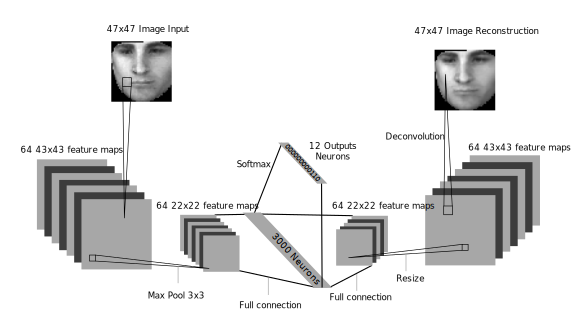
\includegraphics[width=\textwidth]{illustrations/aec_network.pdf}
   \captionof{figure}{A diagram of network \networkII\ described in table \ref{tab:netII}.}
   \label{fig:netII}
  \end{figure}

  \section{Common Parameters}
    In order to develop the network for modelling the DISFA dataset a set of common
    parameters for experimentation are useful to define, these are shown in table \ref{tab:common}
    and are assumed unless stated otherwise in the whole chapter.

    \begin{table}[!h]
      \centering { \footnotesize
      \begin{tabular}{ll}
        \hline
        \textbf{Parameter}                       & \textbf{Value}                \\ \hline
        Optimizer                                & Adam                          \\
        Learning Rate                            & $10^{-3}$                     \\
        L2 Regularisation Coefficient            & 0                             \\
        Hidden layer activation functions        & Leaky ReLu, $\alpha=0.01$     \\
        Image downscaling                        & 0.4 ($47\times47$)        \\
        AU's present                             & 1,2,4,5,6,9,12,15,17,20,25,26 \\
        Iterations:                              & 1000                          \\
        Early model save percent                 & 50\%                          \\
        Weight tensor initial standard deviation & $10^{-3}$                     \\
        Bias tensor initial value                & $10^{-2}$                     \\
        Train batch size                         & 100                           \\
        Validation batch size                    & 500                           \\
        Autoencoder cost function                & Mean Squared Error            \\
        Classifier cost function                 & Cross Entropy                 \\
        \hline
      \end{tabular}
      \caption{Common parameters for most experiments in the section. These parameters should be
      assumed in proceeding sections unless otherwise stated.} \label{tab:common} }
    \end{table}

    The Adam optimizer is a popular choice for deep learning models and has an adaptive learning rate
    so the learning rate is initially set to $10^{-3}$ which is standard. The Leaky ReLu
    has shown small improvements in classification rates so is used as opposed
    to the standard ReLU. Images are downscaled by 0.4 to the resolution $47\times47$
    as in done in some of the networks shown in \ref{tab:compnet}.
    The early model save percent states when the whole model should be saved early,
    this means for each experiment run there are two models to be evaluated. This
    is useful for the evaluation of both autoencoder and classifier training in one go.

    The mean squared error is chosen to train the autoencoder as there are few other alternatives
    and the cross entropy for the classifer as it heavily penalises incorrect classifications,
    unlike the mean squared error.

  \section{Joint classification}

    Typical deep neural networks are used to classify
    one image into only one category. The case with FAU detection is different, we
    would like to be able to classify the categories jointly,  putting one frame into more than
    one AU category. Ideally the network would output a confidence score between 0 and 1
    to signify if an AU is present and we would calculate some optimum threshold value
    (ideally this would be 0.5).

    The following list details three possible solutions to the joint classification problem:

    \begin{itemize} \label{sec:binsoft}
      \item {\bf Softmax Layer} - This is a traditional, fully connected layer with
      a softmax activation function (see equation \ref{eq:softmax}).
      The issue with this is that it provides a probability distribution over AUs
      but the required quantity is a probability distribution for each AU.
      \item {\bf Sigmoid Layer} - This again is like the previous solution but instead each neuron gives a confidence
      score between 0 and 1 for each AU with a sigmoid function (see equation \ref{eq:sigmoid}).
      The issue with this however is that sigmoid
      functions have vanishing gradients at large input values
      hence training may become difficult.
      \item {\bf Binary Softmax Layers} - Here there is a two neuron softmax layer
      for each AU, this doubles the amount of weights
      but gives a probability over the presence and
      absence of each AU which is ideal. In the implementation
      the negative neuron of each binary layer is only used for training purposes, and it is
      discarded while evaluating the classification performance.
    \end{itemize}


  \section{Network Structures}

    % Inspired by the literature (see table \ref{tab:compnet}) four networks are
    % defined. Network \networkII\ is shown in table \ref{tab:net2}, Network
    % \networkII\  adds another convolutional layer of size $5\times 5 \times 64
    % \times 64$ to this and Network \networkIV\ adds a $4\times 4 \times 64 \times
    % 128$ layer on top of Network \networkII. Regarding the decoder section the
    % inverse operations are performed, see appendix \label{appendix1} for full
    % details for networks \networkII, \networkIII\ and \networkIV.

    Network \networkI\, acts as a baseline as it is the simplest
    possible network to incorporate the proposed structure. It is defined in Table~\ref{tab:netI},
    it contains one hidden layer of 12 neurons which is connected to the input image of 2209 pixels,
    the output reconstruction of 2209 pixels and to the classifer, which is shown as the Binary Softmax
    (preempting the results from chapter \ref{chap:Evaluation}). In order to
    use the DISFA images with this network, they are flattened into an array 2209 sized array.
    12 neurons
    are chosen heuristically as there are 12 AU's and one might naively hope that the number of
    neurons required in the hidden layer would be roughly equal to the number of features.

    Network \networkII\ (Table~\ref{tab:netI} and figure \ref{fig:netII}) contains all of the indredients of a deep learning
    algorithm a convolutional layer and secondly a $3\times 3$ max pooling layer.

    Networks \networkIII\ (Table~\ref{tab:netIII}) and \networkIV\ (Table~\ref{tab:netIV})
    build on this by each adding an extra convolutional layer.

    Networks \networkII, \networkIII\ are \networkIV\ based off of networks in
    the literature, but with the aditional decoder section which is achieved by
    using deconvolutional layers. These deconvolutions are actually transposed
    convolutions, so on the final layer in order to reconstruct an image, all of
    the feature maps are averaged together to create
    the final image.

    The cost function of these networks is:

    \begin{equation} \label{eq:l2_cost_model}
        J(\tilde{\mathbf{x}},\tilde{\mathbf{y}}) = -\frac{1-\alpha(t)}{2FN}\tilde{\mathbf{y}}\cdot\log(\mathbf{y}(\tilde{\mathbf{x}}))
        + \frac{\alpha(t)}{N}\left |\mathbf{y}(\tilde{\mathbf{x}}) \odot \mathbf{M}-\tilde{\mathbf{x}}\right | ^2
    \end{equation}

    Where $\mathbf{M}$ is a mask described in section \ref{sec:mask}. Here F is the number of AU's, N is the size of the batch and $\alpha(t)$ is a
    function which balances the two costs and is described in section \ref{sec:autoalpha}.

    % This section shows the network structures used, branching in a network is described
% with an extra column.
% \begin{table}[h!]
%   \caption*{\textbf{Network \networkI}}
% 	\centering
% 	{\footnotesize
% 		\begin{tabular}{|lllllllll|}
% 			\hline
% 			\multicolumn{1}{|l|}{Element} & Type    & \multicolumn{1}{l|}{Dimensions}           & Type           & \multicolumn{1}{l|}{Dimensions}            \\ \hline
% 			\multicolumn{1}{|l|}{x}       &         & \multicolumn{1}{l|}{$47\times47\times1$}  &                & \multicolumn{1}{l|}{}                      \\ \hline
% 			\multicolumn{1}{|l|}{$L_1$}   & flatten + fc      & \multicolumn{1}{l|}{$2209\times12$}       & Binary Softmax & \multicolumn{1}{l|}{$3000\times2\times12$} \\
% 			\multicolumn{1}{|l|}{$y_1$}   & dropout & \multicolumn{1}{l|}{$12$}                 &                & \multicolumn{1}{l|}{$24$}                  \\ \hline
% 			\multicolumn{1}{|l|}{$L_2$}   & fc      & \multicolumn{1}{l|}{$12\times2209$}       &                & \multicolumn{1}{l|}{}                      \\
% 			\multicolumn{1}{|l|}{$y_2$}   &         & \multicolumn{1}{l|}{$3000$}               &                & \multicolumn{1}{l|}{}                      \\ \hline
% 			\multicolumn{1}{|l|}{$L_3$}   & reshape & \multicolumn{1}{l|}{}                     &                & \multicolumn{1}{l|}{}                      \\
% 			\multicolumn{1}{|l|}{$y_3$}   &         & \multicolumn{1}{l|}{$47\times47\times 1$} &                & \multicolumn{1}{l|}{}                      \\ \hline
% 		\end{tabular}
%
% 		\caption{This network is the simplest possible which implements the autoencoder classifier structure.
%     It first flattens the input image, runs it through the first layer to get 12 neuron activations.
%     Then it branches, for the decoder into a layer of size $2209$ which is reshaped into a $47\times47$ reconstruction and for the classifier into 12 pairs of binary softmax layers.
%     *Bottleneck layer} \label{tab:netI}
%
% 	}
% \end{table}
\begin{landscape}
	\begin{table}[h] {\footnotesize
			\centering
			\caption*{\textbf{Network \networkI}}
			\begin{tabular}{lllllllllllllll}
				\cline{1-9}
				\multicolumn{3}{|c|}{Encoder}                                                              & \multicolumn{3}{c|}{Decoder}                                                 & \multicolumn{3}{c|}{Classifier}                                                            &  &  &  &  &  &  \\ \cline{1-9}
				\multicolumn{1}{|l|}{Element} & Type         & \multicolumn{1}{l|}{Dimensions}             & \multicolumn{1}{l|}{Element} & Type    & \multicolumn{1}{l|}{Dimensions}     & \multicolumn{1}{l|}{Element} & Type           & \multicolumn{1}{l|}{Dimensions}            &   &   &   &   &   &   \\ \cline{1-9}
				\multicolumn{1}{|l|}{$x$}     & Input        & \multicolumn{1}{l|}{$47\times 47 \times 1$} & \multicolumn{1}{l|}{$y_1$}   & dropout & \multicolumn{1}{l|}{12}             & \multicolumn{1}{l|}{$y_1$}   & dropout        & \multicolumn{1}{l|}{12}                    &   &   &   &   &   &   \\ \cline{1-9}
				\multicolumn{1}{|l|}{$L_1$}   & flatten + fc & \multicolumn{1}{l|}{$2209\times12$}         & \multicolumn{1}{l|}{$L_2$}   & fc      & \multicolumn{1}{l|}{$12\times2209$} & \multicolumn{1}{l|}{$L_3$}   & Binary Softmax & \multicolumn{1}{l|}{$3000\times2\times12$} &   &   &   &   &   &   \\
				\multicolumn{1}{|l|}{$y_1$}   &              & \multicolumn{1}{l|}{12}                     & \multicolumn{1}{l|}{$y_2$}   & Output  & \multicolumn{1}{l|}{$3000$}         & \multicolumn{1}{l|}{$y_3$}   & Output         & \multicolumn{1}{l|}{24}                    &   &   &   &   &   &   \\ \cline{1-9}
			\end{tabular}}
		\caption{Fully connected layers are denoted as fc, convolutional layers as conv and deconvolutional laters are deconv. Layers $L_i$ output tensors $y_i$. $x$ is the initial input into $L_1$.}
    \label{tab:netI}
	\end{table}

	\begin{table}[h] {\footnotesize
			\centering
			\caption*{\textbf{Network \networkII}}
			\begin{tabular}{lllllllllllllll}
				\cline{1-9}
				\multicolumn{3}{|c|}{Encoder}                                                                      & \multicolumn{3}{c|}{Decoder}                                                 & \multicolumn{3}{c|}{Classifier}                                                            &  &  &  &  &  &  \\ \cline{1-9}
				\multicolumn{1}{|l|}{Element} & Type     & \multicolumn{1}{l|}{Dimensions}                  & \multicolumn{1}{l|}{Element} & Type     & \multicolumn{1}{l|}{Dimensions}                  & \multicolumn{1}{l|}{Element} & Type           & \multicolumn{1}{l|}{Dimensions}            &   &   &   &   &                             &   \\ \cline{1-9}
				\multicolumn{1}{|l|}{$x$}     & Input    & \multicolumn{1}{l|}{$47\times 47 \times 1$}      & \multicolumn{1}{l|}{$y_3$}   & dropout  & \multicolumn{1}{l|}{3000}                        & \multicolumn{1}{l|}{$y_3$}   & dropout        & \multicolumn{1}{l|}{3000}                  &   &   &   &   &                             &   \\ \cline{1-9}
				\multicolumn{1}{|l|}{$L_1$}   & conv 1   & \multicolumn{1}{l|}{$5\times 5\times1\times 64$} & \multicolumn{1}{l|}{$L_4$}   & fc       & \multicolumn{1}{l|}{$3000\times30976$}           & \multicolumn{1}{l|}{$L_7$}   & Binary Softmax & \multicolumn{1}{l|}{$3000\times2\times12$} &   &   &   &   &                             &   \\
				\multicolumn{1}{|l|}{$y_1$}   &          & \multicolumn{1}{l|}{$43\times43\times64$}        & \multicolumn{1}{l|}{$y_4$}   &          & \multicolumn{1}{l|}{$30976$}                     & \multicolumn{1}{l|}{$y_7$}   &                & \multicolumn{1}{l|}{24}                    &   &   &   &   &                             &   \\ \cline{1-9}
				\multicolumn{1}{|l|}{$L_2$}   & max pool & \multicolumn{1}{l|}{$2\times 2$}                 & \multicolumn{1}{l|}{$L_5$}   & reshape  & \multicolumn{1}{l|}{}                            &                              &                & \multicolumn{1}{l}{}                       &   &   &   &   &                             &   \\
				\multicolumn{1}{|l|}{$y_2$}   &          & \multicolumn{1}{l|}{$22\times22\times 64$}       & \multicolumn{1}{l|}{$y_5$}   &          & \multicolumn{1}{l|}{$22\times22\times64$}        &                              &                & \multicolumn{1}{l}{}                       &   &   &   &   &                             &   \\ \cline{1-6}
				\multicolumn{1}{|l|}{$L_3$}   & fc       & \multicolumn{1}{l|}{$30976\times3000$}           & \multicolumn{1}{l|}{$L_6$}   & resize   & \multicolumn{1}{l|}{$2$}                         &                              &                & \multicolumn{1}{l}{}                       &   &   &   &   &                             &   \\
				\multicolumn{1}{|l|}{$y_3$}   & dropout  & \multicolumn{1}{l|}{$3000$}                      & \multicolumn{1}{l|}{$y_6$}   &          & \multicolumn{1}{l|}{$43\times43\times64$}        &                              &                & \multicolumn{1}{l}{}                       &   &   &   &   &                             &   \\ \cline{1-6}
				                              &          &                                                  & \multicolumn{1}{|l|}{$L_7$}  & deconv 1 & \multicolumn{1}{l|}{$5\times 5\times1\times 64$} &                              &                & \multicolumn{1}{l}{}                       &   &   &   &   &                             &   \\
				                              &          &                                                  & \multicolumn{1}{|l|}{$y_7$}  &          & \multicolumn{1}{l|}{$47\times47\times1$}         &                              &                & \multicolumn{1}{l}{}                       &   &   &   &   &                             &   \\ \cline{4-6}
			\end{tabular}}
		\caption{Fully connected layers are denoted as fc, convolutional layers as conv and deconvolutional laters are deconv. Layers $L_i$ output tensors $y_i$. $x$ is the initial input into $L_1$.}
    \label{tab:netII}
	\end{table}


	\begin{table}[h] {\footnotesize
			\centering
			\caption*{\textbf{Network \networkIII}}
			\begin{tabular}{lllllllllllllll}
				\cline{1-9}
				\multicolumn{3}{|c|}{Encoder}                                                                      & \multicolumn{3}{c|}{Decoder}                                                 & \multicolumn{3}{c|}{Classifier}                                                            &  &  &  &  &  &  \\ \cline{1-9}
				\multicolumn{1}{|l|}{Element} & Type     & \multicolumn{1}{l|}{Dimensions}                  & \multicolumn{1}{l|}{Element} & Type     & \multicolumn{1}{l|}{Dimensions}                   & \multicolumn{1}{l|}{Element} & Type           & \multicolumn{1}{l|}{Dimensions}            &   &                             &         &                             &                            &   \\ \cline{1-9}
				\multicolumn{1}{|l|}{$x$}     & Input    & \multicolumn{1}{l|}{$47\times 47 \times 1$}      & \multicolumn{1}{l|}{$y_3$}   & dropout  & \multicolumn{1}{l|}{3000}                         & \multicolumn{1}{l|}{$y_3$}   & dropout        & \multicolumn{1}{l|}{3000}                  &   &                             &         &                             &                            &   \\ \cline{1-9}
				\multicolumn{1}{|l|}{$L_1$}   & conv 1   & \multicolumn{1}{l|}{$5\times 5\times1\times 64$} & \multicolumn{1}{l|}{$L_4$}   & fc       & \multicolumn{1}{l|}{$3000\times20736$}            & \multicolumn{1}{l|}{$L_9$}   & Binary Softmax & \multicolumn{1}{l|}{$3000\times2\times12$} &   &                             &         &                             &                            &   \\
				\multicolumn{1}{|l|}{$y_1$}   &          & \multicolumn{1}{l|}{$43\times43\times64$}        & \multicolumn{1}{l|}{$y_4$}   &          & \multicolumn{1}{l|}{$20736$}                      & \multicolumn{1}{l|}{$y_9$}   &                & \multicolumn{1}{l|}{24}                    &   &                             &         &                             &                            &   \\ \cline{1-9}
				\multicolumn{1}{|l|}{$L_2$}   & max pool & \multicolumn{1}{l|}{$2\times 2$}                 & \multicolumn{1}{l|}{$L_5$}   & reshape  & \multicolumn{1}{l|}{}                             &                              &                & \multicolumn{1}{l}{}                       &   &                             &         &                             &                            &   \\
				\multicolumn{1}{|l|}{$y_2$}   &          & \multicolumn{1}{l|}{$22\times22\times 64$}       & \multicolumn{1}{l|}{$y_5$}   &          & \multicolumn{1}{l|}{$18\times18\times64$}         &                              &                & \multicolumn{1}{l}{}                       &   &                             &         &                             &                            &   \\ \cline{1-6}
				\multicolumn{1}{|l|}{$L_3$}   & conv 2   & \multicolumn{1}{l|}{$5\times 5\times1\times 64$} & \multicolumn{1}{l|}{$L_7$}   & deconv 2 & \multicolumn{1}{l|}{$5\times 5\times64\times 64$} &                              &                & \multicolumn{1}{l}{}                       &   &                             &         &                             &                            &   \\
				\multicolumn{1}{|l|}{$y_3$}   &          & \multicolumn{1}{l|}{$18\times18\times64$}        & \multicolumn{1}{l|}{$y_7$}   &          & \multicolumn{1}{l|}{$22\times22\times64$}         &                              &                & \multicolumn{1}{l}{}                       &   &                             &         &                             &                            &   \\ \cline{1-6}
				\multicolumn{1}{|l|}{$L_3$}   & fc       & \multicolumn{1}{l|}{$20736\times3000$}           & \multicolumn{1}{l|}{$L_6$}   & resize   & \multicolumn{1}{l|}{$2$}                          &                              &                & \multicolumn{1}{l}{}                       &   &                             &         &                             &                            &   \\
				\multicolumn{1}{|l|}{$y_3$}   & dropout  & \multicolumn{1}{l|}{$3000$}                      & \multicolumn{1}{l|}{$y_6$}   &          & \multicolumn{1}{l|}{$43\times43\times64$}         &                              &                & \multicolumn{1}{l}{}                       &   &                             &         &                             &                            &   \\ \cline{1-6}
				                              &          &                                                  & \multicolumn{1}{|l|}{$L_8$}  & deconv 1 & \multicolumn{1}{l|}{$5\times 5\times1\times 64$}  &                              &                & \multicolumn{1}{l}{}                       &   &                             &         &                             &                            &   \\
				                              &          &                                                  & \multicolumn{1}{|l|}{$y_8$}  &          & \multicolumn{1}{l|}{$47\times47\times1$}          &                              &                & \multicolumn{1}{l}{}                       &   &                             &         &                             &                            &   \\ \cline{4-6}
			\end{tabular}}
		\caption{Fully connected layers are denoted as fc, convolutional layers as conv and deconvolutional laters are deconv. Layers $L_i$ output tensors $y_i$. $x$ is the initial input into $L_1$.}
    \label{tab:netIII}
	\end{table}


	\begin{table}[h] {\footnotesize
			\centering
			\caption*{\textbf{Network \networkIV}}
			\begin{tabular}{lllllllllllllll}
				\cline{1-9}
				\multicolumn{3}{|c|}{Encoder}                                                                      & \multicolumn{3}{c|}{Decoder}                                                 & \multicolumn{3}{c|}{Classifier}                                                            &  &  &  &  &  &  \\ \cline{1-9}
				\multicolumn{1}{|l|}{Element} & Type     & \multicolumn{1}{l|}{Dimensions}                  & \multicolumn{1}{l|}{Element} & Type     & \multicolumn{1}{l|}{Dimensions}                    & \multicolumn{1}{l|}{Element} & Type           & \multicolumn{1}{l|}{Dimensions}            &   &                             &   &                                           &                            &   \\ \cline{1-9}
				\multicolumn{1}{|l|}{$x$}     & Input    & \multicolumn{1}{l|}{$47\times 47 \times 1$}      & \multicolumn{1}{l|}{$y_3$}   & dropout  & \multicolumn{1}{l|}{3000}                          & \multicolumn{1}{l|}{$y_3$}   & dropout        & \multicolumn{1}{l|}{3000}                  &   &                             &   &                                           &                            &   \\ \cline{1-9}
				\multicolumn{1}{|l|}{$L_1$}   & conv 1   & \multicolumn{1}{l|}{$5\times 5\times1\times 64$} & \multicolumn{1}{l|}{$L_4$}   & fc       & \multicolumn{1}{l|}{$3000\times14400$}             & \multicolumn{1}{l|}{$L_7$}   & Binary Softmax & \multicolumn{1}{l|}{$3000\times2\times12$} &   &                             &   &                                           &                            &   \\
				\multicolumn{1}{|l|}{$y_1$}   &          & \multicolumn{1}{l|}{$43\times43\times64$}        & \multicolumn{1}{l|}{$y_4$}   &          & \multicolumn{1}{l|}{$14400$}                       & \multicolumn{1}{l|}{$y_7$}   &                & \multicolumn{1}{l|}{24}                    &   &                             &   &                                           &                            &   \\ \cline{1-9}
				\multicolumn{1}{|l|}{$L_2$}   & max pool & \multicolumn{1}{l|}{$2\times 2$}                 & \multicolumn{1}{l|}{$L_5$}   & reshape  & \multicolumn{1}{l|}{}                              &                              &                & \multicolumn{1}{l}{}                       &   &                             &   &                                           &                            &   \\
				\multicolumn{1}{|l|}{$y_2$}   &          & \multicolumn{1}{l|}{$22\times22\times 64$}       & \multicolumn{1}{l|}{$y_5$}   &          & \multicolumn{1}{l|}{$15\times15\times64$}          &                              &                & \multicolumn{1}{l}{}                       &   &                             &   &                                           &                            &   \\ \cline{1-6}
				\multicolumn{1}{|l|}{$L_3$}   & conv 2   & \multicolumn{1}{l|}{$5\times 5\times1\times 64$} & \multicolumn{1}{l|}{$L_6$}   & deconv 3 & \multicolumn{1}{l|}{$5\times 5\times64\times 64$}  &                              &                & \multicolumn{1}{l}{}                       &   &                             &   &                                           &                            &   \\
				\multicolumn{1}{|l|}{$y_3$}   &          & \multicolumn{1}{l|}{$18\times18\times64$}        & \multicolumn{1}{l|}{$y_6$}   &          & \multicolumn{1}{l|}{$18\times18\times64$}          &                              &                & \multicolumn{1}{l}{}                       &   &                             &   &                                           &                            &   \\ \cline{1-6}
				\multicolumn{1}{|l|}{$L_3$}   & conv 3   & \multicolumn{1}{l|}{$5\times 5\times1\times 64$} & \multicolumn{1}{l|}{$L_7$}   & deconv 2 & \multicolumn{1}{l|}{$5\times 5\times64\times 64$}  &                              &                & \multicolumn{1}{l}{}                       &   &                             &   &                                           &                            &   \\
				\multicolumn{1}{|l|}{$y_3$}   &          & \multicolumn{1}{l|}{$15\times15\times64$}        & \multicolumn{1}{l|}{$y_7$}   &          & \multicolumn{1}{l|}{$22\times22\times64$}          &                              &                & \multicolumn{1}{l}{}                       &   &                             &   &                                           &                            &   \\ \cline{1-6}
				\multicolumn{1}{|l|}{$L_3$}   & fc       & \multicolumn{1}{l|}{$14400\times3000$}           & \multicolumn{1}{l|}{$L_8$}   & resize   & \multicolumn{1}{l|}{$2$}                           &                              &                & \multicolumn{1}{l}{}                       &   &                             &   &                                           &                            &   \\
				\multicolumn{1}{|l|}{$y_3$}   & dropout  & \multicolumn{1}{l|}{$3000$}                      & \multicolumn{1}{l|}{$y_8$}   &          & \multicolumn{1}{l|}{$43\times43\times64$}          &                              &                & \multicolumn{1}{l}{}                       &   &                             &   &                                           &                            &   \\ \cline{1-6}
				                              &          &                                                  & \multicolumn{1}{|l|}{$L_9$}  & deconv 1 & \multicolumn{1}{l|}{$5\times 5\times1\times 64$}   &                              &                & \multicolumn{1}{l}{}                       &   &                             &   &                                           &                            &   \\
				                              &          &                                                  & \multicolumn{1}{|l|}{$y_9$}  &          & \multicolumn{1}{l|}{$47\times47\times1$} &                              &                & \multicolumn{1}{l}{}                       &   &                             &   &                                           &                            &   \\ \cline{4-6}
			\end{tabular} }
			\caption{Fully connected layers are denoted as fc, convolutional layers as conv and deconvolutional laters are deconv. Layers $L_i$ output tensors $y_i$. $x$ is the initial input into $L_1$.}
      \label{tab:netIV}
	\end{table}


	%
	% \begin{table}[]
	% \centering
	% \caption*{\textbf{Network \networkII}}
	% \label{my-label}
	% \begin{tabular}{lllllllllllllll}
	% \cline{1-9}
	% \multicolumn{3}{|c|}{Encoder}                                                                      & \multicolumn{3}{c|}{Decoder}                                                 & \multicolumn{3}{c|}{Classifier}                                                            &  &  &  &  &  &  \\ \cline{1-9}
	% \multicolumn{1}{|l|}{Element} & Type         & \multicolumn{1}{l|}{Dimensions}                     & \multicolumn{1}{l|}{Element} & Type    & \multicolumn{1}{l|}{Dimensions}     & \multicolumn{1}{l|}{Element} & Type           & \multicolumn{1}{l|}{Dimensions}            &  &  &  &  &  &  \\ \cline{1-9}
	% \multicolumn{1}{|l|}{$x$}     & Input        & \multicolumn{1}{l|}{$47\times 47 \times 1$}         & \multicolumn{1}{l|}{$y_3$}   & dropout & \multicolumn{1}{l|}{3000}             & \multicolumn{1}{l|}{$y_3$}   & dropout        & \multicolumn{1}{l|}{3000}                    &  &  &  &  &  &  \\ \cline{1-9}
	% \multicolumn{1}{|l|}{$L_1$}   & conv 1           & \multicolumn{1}{l|}{$5\times 5\times1\times 64$}& \multicolumn{1}{l|}{$L_5$}   & fc               & \multicolumn{1}{l|}{$3000\times20736$}           & \multicolumn{1}{l|}{$L_7$}   & Binary Softmax & \multicolumn{1}{l|}{$3000\times2\times12$} &  &  &  &  &  &  \\
	% \multicolumn{1}{|l|}{$y_1$}   &                  & \multicolumn{1}{l|}{$43\times43\times64$}       & \multicolumn{1}{l|}{$y_5$}   &                  & \multicolumn{1}{l|}{$3000$}                      & \multicolumn{1}{l|}{$y_7$}   & & \multicolumn{1}{l|}{24}                    &  &  &  &  &  &  \\ \cline{1-9}
	% \multicolumn{1}{|l|}{$L_2$}   & max pool         & \multicolumn{1}{l|}{$2\times 2$}                & \multicolumn{1}{l|}{$L_6$}   & resize\& reshape & \multicolumn{1}{l|}{$2$}                         &                              & & \multicolumn{1}{l}{} &  &  &  &  &  &  \\
	% \multicolumn{1}{|l|}{$y_2$}   &                  & \multicolumn{1}{l|}{$22\times22\times 64$}      & \multicolumn{1}{l|}{$y_6$}   &                  & \multicolumn{1}{l|}{$18\times18\times 64$}       &                              & & \multicolumn{1}{l}{}                    &  &  &  &  &  &  \\ \cline{1-6}
	% \multicolumn{1}{|l|}{$L_3$}   & conv 2           & \multicolumn{1}{l|}{$5\times 5\times1\times 64$}& \multicolumn{1}{l|}{$L_7$}   & deconv 2         & \multicolumn{1}{l|}{$5\times 5\times64\times 64$} &                               & & \multicolumn{1}{l}{} &  &  &  &  &  &  \\
	% \multicolumn{1}{|l|}{$y_3$}   &                  & \multicolumn{1}{l|}{$18\times18\times64$}       & \multicolumn{1}{l|}{$y_7$}   &                  & \multicolumn{1}{l|}{$22\times22\times64$}        &                              & & \multicolumn{1}{l}{}                    &  &  &  &  &  &  \\ \cline{1-6}
	% \multicolumn{1}{|l|}{$L_3$}   & fc               & \multicolumn{1}{l|}{$30976\times3000$}          & \multicolumn{1}{l|}{$L_8$}   & deconv 1         & \multicolumn{1}{l|}{$5\times 5\times1\times 64$} &                               & & \multicolumn{1}{l}{} &  &  &  &  &  &  \\
	% \multicolumn{1}{|l|}{$y_3$}   & dropout          & \multicolumn{1}{l|}{$3000$}                     & \multicolumn{1}{l|}{$y_8$}   &                  & \multicolumn{1}{l|}{$47\times47\times1$}         &                              & & \multicolumn{1}{l}{}                    &  &  &  &  &  &  \\ \cline{1-6}
	% \end{tabular}
	% \caption{TODO}
	% \end{table}
	%
	%
	% \begin{table}[]
	% \centering
	% \caption*{\textbf{Network \networkII}}
	% \label{my-label}
	% \begin{tabular}{lllllllllllllll}
	% \cline{1-9}
	% \multicolumn{3}{|c|}{Encoder}                                                                      & \multicolumn{3}{c|}{Decoder}                                                 & \multicolumn{3}{c|}{Classifier}                                                            &  &  &  &  &  &  \\ \cline{1-9}
	% \multicolumn{1}{|l|}{Element} & Type         & \multicolumn{1}{l|}{Dimensions}                     & \multicolumn{1}{l|}{Element} & Type    & \multicolumn{1}{l|}{Dimensions}     & \multicolumn{1}{l|}{Element} & Type           & \multicolumn{1}{l|}{Dimensions}            &  &  &  &  &  &  \\ \cline{1-9}
	% \multicolumn{1}{|l|}{$x$}     & Input        & \multicolumn{1}{l|}{$47\times 47 \times 1$}         & \multicolumn{1}{l|}{$y_3$}   & dropout & \multicolumn{1}{l|}{3000}             & \multicolumn{1}{l|}{$y_3$}   & dropout        & \multicolumn{1}{l|}{3000}                    &  &  &  &  &  &  \\ \cline{1-9}
	% \multicolumn{1}{|l|}{$L_1$}   & conv 1           & \multicolumn{1}{l|}{$5\times 5\times1\times 64$}& \multicolumn{1}{l|}{$L_5$}   & fc               & \multicolumn{1}{l|}{$3000\times20736$}           & \multicolumn{1}{l|}{$L_7$}   & Binary Softmax & \multicolumn{1}{l|}{$3000\times2\times12$} &  &  &  &  &  &  \\
	% \multicolumn{1}{|l|}{$y_1$}   &                  & \multicolumn{1}{l|}{$43\times43\times64$}       & \multicolumn{1}{l|}{$y_5$}   &                  & \multicolumn{1}{l|}{$3000$}                      & \multicolumn{1}{l|}{$y_7$}   & & \multicolumn{1}{l|}{24}                    &  &  &  &  &  &  \\ \cline{1-9}
	% \multicolumn{1}{|l|}{$L_2$}   & max pool         & \multicolumn{1}{l|}{$2\times 2$}                & \multicolumn{1}{l|}{$L_6$}   & deconv 3         & \multicolumn{1}{l|}{$5\times 5\times64\times 64$}  &                              & & \multicolumn{1}{l}{} &  &  &  &  &  &  \\
	% \multicolumn{1}{|l|}{$y_2$}   &                  & \multicolumn{1}{l|}{$22\times22\times 64$}      & \multicolumn{1}{l|}{$y_6$}   &                  & \multicolumn{1}{l|}{$22\times22\times64$}          &                              & & \multicolumn{1}{l}{}                    &  &  &  &  &  &  \\ \cline{1-6}
	% \multicolumn{1}{|l|}{$L_3$}   & conv 2           & \multicolumn{1}{l|}{$5\times 5\times1\times 64$}& \multicolumn{1}{l|}{$L_7$}   & resize\& reshape & \multicolumn{1}{l|}{$2$}                       &                               & & \multicolumn{1}{l}{} &  &  &  &  &  &  \\
	% \multicolumn{1}{|l|}{$y_3$}   &                  & \multicolumn{1}{l|}{$18\times18\times64$}       & \multicolumn{1}{l|}{$y_7$}   &                  & \multicolumn{1}{l|}{$18\times18\times 64$}     &                              & & \multicolumn{1}{l}{}                    &  &  &  &  &  &  \\ \cline{1-6}
	% \multicolumn{1}{|l|}{$L_3$}   & conv 3           & \multicolumn{1}{l|}{$5\times 5\times1\times 64$}& \multicolumn{1}{l|}{$L_7$}   & deconv 2         & \multicolumn{1}{l|}{$5\times 5\times64\times 64$}&                               & & \multicolumn{1}{l}{} &  &  &  &  &  &  \\
	% \multicolumn{1}{|l|}{$y_3$}   &                  & \multicolumn{1}{l|}{$18\times18\times64$}       & \multicolumn{1}{l|}{$y_7$}   &                  & \multicolumn{1}{l|}{$43\times43\times64$}        &                              & & \multicolumn{1}{l}{}                    &  &  &  &  &  &  \\ \cline{1-6}
	% \multicolumn{1}{|l|}{$L_3$}   & fc               & \multicolumn{1}{l|}{$30976\times3000$}          & \multicolumn{1}{l|}{$L_8$}   & deconv 1         & \multicolumn{1}{l|}{$5\times 5\times64\times 1$} &                               & & \multicolumn{1}{l}{} &  &  &  &  &  &  \\
	% \multicolumn{1}{|l|}{$y_3$}   & dropout          & \multicolumn{1}{l|}{$3000$}                     & \multicolumn{1}{l|}{$y_8$}   &                  & \multicolumn{1}{l|}{$47\times47\times1$}         &                              & & \multicolumn{1}{l}{}                    &  &  &  &  &  &  \\ \cline{1-6}
	% \end{tabular}
	% \caption{TODO}
	% \end{table}

\end{landscape}
%
% \begin{table}[h!]
% 	\centering
% 	\caption*{\textbf{Network \networkIV}}
% 	{\footnotesize
% 		\begin{tabular}{|lllllllll|}
% 			\hline
% 			\multicolumn{1}{|l|}{Element} & Type             & \multicolumn{1}{l|}{Dimensions}                  & Type           & \multicolumn{1}{l|}{Dimensions}            \\ \hline
% 			\multicolumn{1}{|l|}{x}       &                  & \multicolumn{1}{l|}{$47\times47\times1$}         &                & \multicolumn{1}{l|}{}                      \\ \hline
% 			\multicolumn{1}{|l|}{$L_1$}   & conv 1           & \multicolumn{1}{l|}{$5\times 5\times1\times 64$} &                & \multicolumn{1}{l|}{}                      \\
% 			\multicolumn{1}{|l|}{$y_1$}   &                  & \multicolumn{1}{l|}{$43\times43\times64$}        &                & \multicolumn{1}{l|}{}                      \\ \hline
% 			\multicolumn{1}{|l|}{$L_2$}   & max pool         & \multicolumn{1}{l|}{$2\times 2$}                 &                & \multicolumn{1}{l|}{}                      \\
% 			\multicolumn{1}{|l|}{$y_2$}   &                  & \multicolumn{1}{l|}{$22\times22\times 64$}       &                & \multicolumn{1}{l|}{}                      \\ \hline
% 			\multicolumn{1}{|l|}{$L_3$}   & conv 2           & \multicolumn{1}{l|}{$5\times 5\times1\times 64$} &                & \multicolumn{1}{l|}{}                      \\
% 			\multicolumn{1}{|l|}{$y_3$}   &                  & \multicolumn{1}{l|}{$18\times18\times64$}        &                & \multicolumn{1}{l|}{}                      \\ \hline
% 			\multicolumn{1}{|l|}{$L_4$}   & conv 3           & \multicolumn{1}{l|}{$5\times 5\times1\times 64$} &                & \multicolumn{1}{l|}{}                      \\
% 			\multicolumn{1}{|l|}{$y_4$}   &                  & \multicolumn{1}{l|}{$15\times15\times64$}        &                & \multicolumn{1}{l|}{}                      \\ \hline
% 			\multicolumn{1}{|l|}{$L_5$}   & fc               & \multicolumn{1}{l|}{$14400\times3000$}           & Binary Softmax & \multicolumn{1}{l|}{$3000\times2\times12$} \\
% 			\multicolumn{1}{|l|}{$y_5$}   & dropout          & \multicolumn{1}{l|}{$3000$}                      &                & \multicolumn{1}{l|}{$24$}                  \\ \hline
% 			\multicolumn{1}{|l|}{$L_6$}   & fc               & \multicolumn{1}{l|}{$3000\times 14400$}          &                & \multicolumn{1}{l|}{}                      \\
% 			\multicolumn{1}{|l|}{$y_6$}   &                  & \multicolumn{1}{l|}{$3000$}                      &                & \multicolumn{1}{l|}{}                      \\ \hline
% 			\multicolumn{1}{|l|}{$L_7$}   & resize\& reshape & \multicolumn{1}{l|}{$2$}                         &                & \multicolumn{1}{l|}{}                      \\
% 			\multicolumn{1}{|l|}{$y_7$}   &                  & \multicolumn{1}{l|}{$15\times15\times 64$}       &                & \multicolumn{1}{l|}{}                      \\ \hline
% 			\multicolumn{1}{|l|}{$L_8$}   & deconv 3         & \multicolumn{1}{l|}{$5\times 5\times1\times 64$} &                & \multicolumn{1}{l|}{}                      \\
% 			\multicolumn{1}{|l|}{$y_8$}   &                  & \multicolumn{1}{l|}{$18\times18\times64$}        &                & \multicolumn{1}{l|}{}                      \\ \hline
% 			\multicolumn{1}{|l|}{$L_9$}   & deconv 2         & \multicolumn{1}{l|}{$5\times 5\times1\times 64$} &                & \multicolumn{1}{l|}{}                      \\
% 			\multicolumn{1}{|l|}{$y_9$}   &                  & \multicolumn{1}{l|}{$22\times22\times64$}        &                & \multicolumn{1}{l|}{}                      \\ \hline
% 			\multicolumn{1}{|l|}{$L_{10}$}   & deconv 1         & \multicolumn{1}{l|}{$5\times 5\times1\times 64$} &                & \multicolumn{1}{l|}{}                      \\
% 			\multicolumn{1}{|l|}{$y_{10}$}   &                  & \multicolumn{1}{l|}{$47\times47\times1$}         &                & \multicolumn{1}{l|}{}                      \\ \hline
% 		\end{tabular}
% 		\caption{ \newline *Bottleneck layer} \label{tab:netIV}
% 	}
% \end{table}


  \clearpage


  \section{Sharing Weights}
    In order to reduce the number of parameters in an autoencoder, to avoid over
    fitting and the probability of learning the identity function, it is often
    helpful to share weights between the encoder and decoder sections (see section
    \ref{sec:autoencoders}).

    In this implementation this is done only for the weights and not the biases,
    the weights for the paired layers are related by their transposes.
  \section{Local Contrast Normalisation}
    Local Contrast Normalisation was implemented as described in section \ref{sec:lrn} with
    constants $k=2,n=5,\alpha=10^{-4}$ and $\beta=0.75$.
    It was applied differently for each network, as follows:
    \begin{itemize}
      \item Network \networkI   : not possible as no convolutional layers
      \item Network \networkII  : applied onto $y_2$ and fed into $L_3$
      \item Network \networkIII : applied onto $y_2$ and fed into $L_3$ and applied onto $y_3$ and fed into $L_4$
      \item Network \networkIV  : applied onto $y_2$ and fed into $L_3$ and applied onto $y_5$ and fed into $L_5$
    \end{itemize}
  \section{Dropout}
    All of the networks contain dropout, although in different experiments it's
    value is between 0.8 and 1 (this is the probability of a neuron staying
    active). Dropout is always at the bottleneck layer, the layer which
    connnects to the encoder, decoder and classifiers.
  \section{L2 Regularisation}
    L2 Regularisation incurs a penalty to using weights which have high values.
    This was implemented by adding L2 loss terms for all weight variables. The
    new cost function becomes:

    \begin{equation} \label{eq:l2_cost_model}
        J(\tilde{\mathbf{x}},\tilde{\mathbf{y}}) = -\frac{1-\alpha(t)}{2FN}\tilde{\mathbf{y}}\cdot\log(\mathbf{y}(\tilde{\mathbf{x}}))
        + \frac{\alpha(t)}{N}\left |\mathbf{y}(\tilde{\mathbf{x}}) \odot \mathbf{M}-\tilde{\mathbf{x}}\right | ^2
        + \beta \sum_i^{\text{weights}}||\mathbf{W}_i||^2
    \end{equation}

    Where $\beta$ is some positive balancing factor and $\mathbf{W}$ signifies
    a weight tensor from any type of layer in the network.



  \section{Autoencoder classifier balancing}
    \label{sec:autoalpha}
    In order to generalise the concept of pre-training the following function is used:

    \begin{equation}
      J(\tilde{\mathbf{x}},\tilde{\mathbf{y}}) = -\frac{1-\alpha(t)}{2FN_B}\tilde{\mathbf{y}}\cdot\log(\mathbf{y}(\tilde{\mathbf{x}}))
      + \frac{\alpha(t)}{N_BN_P}\left |\mathbf{y}(\tilde{\mathbf{x}}) \odot \mathbf{M}-\tilde{\mathbf{x}}\right | ^2
    \end{equation}

    The function $\alpha(t)$ might be constant $\left ( \alpha_{\text{constant}}(t)=\frac{1}{2} \right )$ or
    some sort of polynomial which stays in the range $[0,1]$. $N_B$ and $N_P$ are the batch size and number of pixels respectively.

    For much of the initial investigations we employ:
    \begin{equation}
      \alpha_{\text{step}}(t,p,T) =
      \begin{cases}
        1           & \text{if}\ t<pT \\
        0           & \text{otherwise}
      \end{cases}
    \end{equation}

    Where $t$ indexes iterations, $T$ is the total number of iterations and p is the
    percentage of iterations that should be in the first region of the piecewise function
    where $\alpha=1$.
    This nicely expresses what is typically meant by pre-training in the literature, it trains
    the autoencoder up until iteration $pT$ (normally $p=\frac{1}{2}$ or $p=\frac{2}{3}$) and then the classifier for the remainder of the time.
    This acts as a good base case to test both sides of the network, later more interesting
    functions will be explored such as the sigmoid step:

    \begin{equation}
      \alpha_{\text{sigmoid}}(t,T,p,\tau) = \frac{1}{1 + \exp(1 + \tau (t/T - p))}
    \end{equation}

    Or a polynomial function:

    \begin{equation}
      \alpha_{\text{poly}}(t,T,n) = 1 - \left ( \frac{t}{T} \right )^n
    \end{equation}

    Or a periodic step function:

    \begin{equation}
      \alpha_{\text{alternate}}(t,T,p) =
      \begin{cases}
        1           & \text{if } t < |T/p| \text{ and } p > 0\\
        0           & \text{if } t < |T/p| \text{ and } p \leq 0\\
        \alpha_{\text{alternate}}(t-|T/p|,T,-p)           & \text{otherwise} \\
      \end{cases}
    \end{equation}

    Examples of such functions are plotted in figure \ref{fig:alpha_functions}.

    \begin{figure}[!h]
      \centering
      \includegraphics[width =\hsize]{figures/alpha.pdf}
      \caption{Examples of branch balancing functions described in section \ref{sec:autoalpha}.
      For the polynomial case higher values of $n$ decrease the amount of training
      the classifier receives. While in the case of the step p dictates the training
      that each network receives, the sigmoid can be seen as a smoothed out step function
      with the two being equivalent as $ \tau \rightarrow \infty$. Similarly as $n \rightarrow \infty$
      the polynomial function turns into a constant function with $c=1$ except at the final
      iteration.}
      \label{fig:alpha_functions}
    \end{figure}
